\documentclass{article}

\usepackage{fancyhdr}
\usepackage[parfill]{parskip}
\usepackage{graphicx}

\pagestyle{fancyplain}

\author{Todd Davies}
\title{3.2.2 DNA}
\date{\today}

\begin{document}

\rhead{3.5.7 Gene expression}
\lhead{\today}

\maketitle

\subsection*{Promotor regions}
\thispagestyle{empty}

For transcription to take place, RNA polymerase must attach to DNA near the gene
to be translated. Promotor regions are sections of DNA that are situated near
genes that allow transcription factors to bind to the DNA.

\section*{Transcription factors}

Transcription factors bind to promotor regions on genes. Their role is to
attract an RNA polymerase enzyme so that mRNA can be produced.

Transcription factors are often second messengers (such as cAMP). Their role is
to initialise protein synthesis within the cell by starting transcription
process of the gene that codes for the protein inside the nucleus.

\begin{figure}
	\centering
	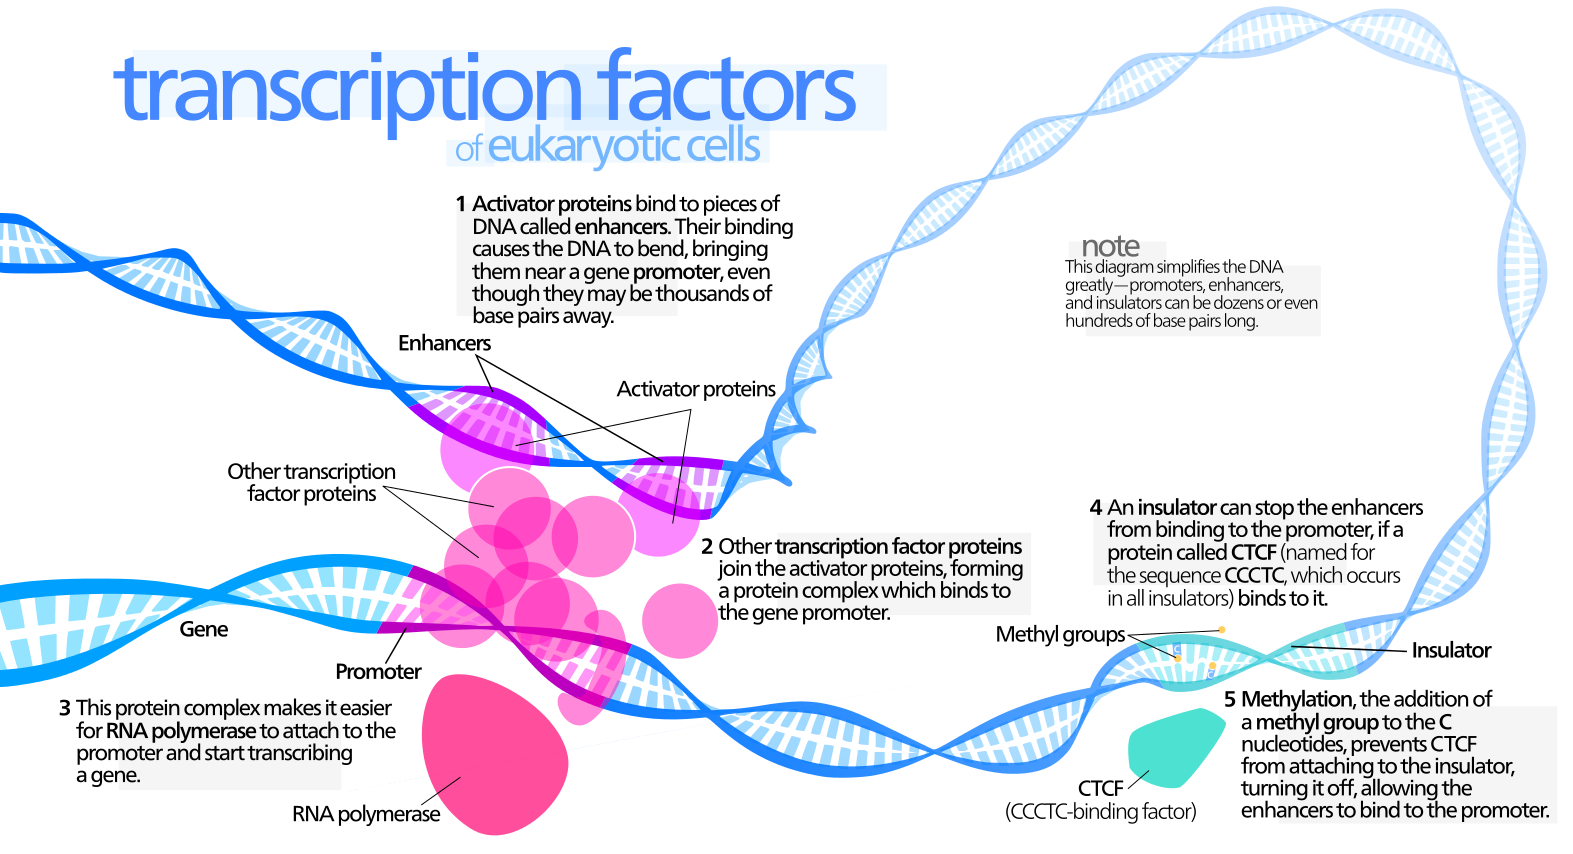
\includegraphics[scale=0.3, angle=90]{transcriptionfactors}
\end{figure}

\newpage

\section*{Small Interfering RNA}

Small interfering RNA (siRNA) is a double stranded section of RNA about 20-25
bases long that interferes with the expression of specific genes.

Their bases are complementary to specific sections of a specific gene The siRNA
can interfere with both the translation and transcription of the gene.

When if affects translation, a mechanism called {\it RNA interference} occurs.
This involves siRNA binding and other proteins binding to target mRNA in the
cytoplasm and then proteins cutting the mRNA into sections so that the gene
cannot be expressed.

\end{document}
